\section{An exact construction with rational target witnesses}
\label{sec:target-algorithm}
We now construct the certificate of \cref{thm:universal}. The implementation deliberately uses a transparent vertical-slice method rather than an optimal arrangement data structure. Its witness list can be checked using rational point membership alone.

\subsection{Critical abscissae}
Include the following real numbers in a list $X$:
\begin{enumerate}
\item the first coordinates of every target vertex;
\item the leftmost and rightmost first coordinates $c_{i,x}\pm r_i$ of each disk;
\item the first coordinates of every intersection of two distinct supporting circles;
\item the first coordinates of every intersection of a circle with a target-edge segment;
\item the first coordinates of every intersection of two target-edge segments.
\end{enumerate}
Remove duplicates and numbers outside the horizontal span of the target. Pairwise coincidences create no infinite list: coincident circle boundaries are represented once for ordering, while contact labels remain distinct; overlapping collinear segments need only their endpoints. Their order does not exchange inside an open slab.

There are $O((n+h)^2)$ listed numbers. Each is rational or has the form $a+b\sqrt d$ with $a,b,d\in\mathbb Q$ and $d\ge0$. Circle--circle formulas are derived in \cref{sec:geometry}. For a segment $p+t(q-p)$, circle intersection is a quadratic equation in $t$, retaining roots in $[0,1]$. Segment intersections have rational coordinates.

For each consecutive pair $\alpha<\beta$ in $X$, choose a rational $x_0\in(\alpha,\beta)$. The vertical line at $x_0$ meets a circle, when appropriate, at
\[
y=c_{i,y}\pm\sqrt{r_i^2-(x_0-c_{i,x})^2},
\]
and a nonvertical target edge at a rational ordinate. Sort these ordinates exactly, remove duplicate values and choose a rational ordinate between every consecutive pair. Test the resulting point for membership in the target interior and, if retained, compute its exact contact mask.

The target is bounded, so every interior component of its vertical section is bracketed by target-edge intersections. Sampling the two unbounded ordinate intervals is unnecessary. Vertical target edges lie on critical abscissae; their omission from generic sections is justified by \cref{lem:interior-witness}, rather than by assuming they have no target points.

\begin{theorem}[Completeness of vertical sampling]\label{thm:sweep}
The construction visits a point in every two-dimensional arrangement cell that meets the target interior. After taking inclusion-minimal contact masks, it returns exactly $\mathcal A_T$ with rational witnesses. It also applies to any fixed monotone activation map $\gamma$, returning the minimal mapped masks.
\end{theorem}
\begin{proof}
Between consecutive critical abscissae, no circle appears or disappears in a vertical section, no target-edge segment begins or ends, and two section curves cannot exchange their order. Such an exchange would require an intersection whose first coordinate belongs to $X$. Equal section curves can persist, as with coincident circles or overlapping segments; keeping one ordinate for a persistent equality leaves every open band represented.

Thus each open ordinate band continues through the slab without a boundary crossing, and its contact labels and target membership are constant. Choosing one rational point per band gives those labels exactly. Conversely every two-dimensional target cell has an open horizontal projection, which cannot be contained in the finite list $X$. It therefore meets some open slab and one of its bands. Its mask is among the samples. \Cref{thm:universal} identifies the minimal masks with $\mathcal A_T$. For an activation map, apply \cref{thm:relabel}, or evaluate that map on every sample before minimalization.
\end{proof}

\subsection{Comparing two quadratic numbers}
Numerical square roots are not needed even to sort the critical coordinates. Let
\[
x=a+b\sqrt h,\qquad y=c+d\sqrt k,\qquad h,k\ge0.
\]
Set $A=a-c$, $U=A+b\sqrt h$ and $V=d\sqrt k$. We seek the sign of $U-V$.

\begin{lemma}[Two-radical comparison]\label{lem:two-radicals}
The sign of $x-y$ is obtained using rational arithmetic and the one-radical sign test of \cref{lem:sign}. If $U$ and $V$ have different signs, their order follows from those signs. If both are zero, the difference is zero. If their common sign is $s\in\{-1,1\}$, then
\begin{equation}\label{eq:two-radical-comparison}
\operatorname{sgn}(x-y)=s\,\operatorname{sgn}\left(A^2+b^2h-d^2k+2Ab\sqrt h\right).
\end{equation}
\end{lemma}
\begin{proof}
The cases with different signs or both zero are immediate. When $U,V$ are both positive, squaring preserves their order, and $U^2-V^2$ is the expression in parentheses. When both are negative, their order is the reverse of the order of their squares. This gives the factor $s$ and proves the formula, including equality. The sign of $U$ uses one radical, and the sign of $V$ is the sign of $d$ unless $k=0$.
\end{proof}

This test detects equal values with different representations, such as $\sqrt8=2\sqrt2$. It avoids an interval-refinement loop that would never separate two equal algebraic numbers.\footnote{The comparator is a Boolean exactness component, not a numerical approximation routine. An approximate coordinate may still be used for plotting after its role in the certificate has been completed.}

\subsection{Constructing a rational point between algebraic endpoints}
For $h=p/q\ge0$ and an integer precision $b\ge1$, compute
\[
m=\left\lfloor\sqrt{\left\lfloor\frac{p2^{2b}}q\right\rfloor}\right\rfloor.
\]
Then $m/2^b\le\sqrt h<(m+1)/2^b$, unless exact equality holds at the lower endpoint, which is checked by squaring integers. Multiplication by the signed rational coefficient and addition of the rational part give an enclosing rational interval for $a+b'\sqrt h$.

For two strictly ordered endpoints, refine their enclosures until the upper endpoint of the left enclosure is less than the lower endpoint of the right enclosure. Their rational midpoint is the desired sample. The enclosures shrink to distinct real numbers, so the process terminates. All comparisons certifying the selected point are exact. The same routine is used for horizontal and vertical samples.

\begin{proposition}[Operation counts and retained size]\label{prop:sweep-complexity}
Put $M=n+h$. The stated construction has $O(M^2)$ critical abscissae, examines $O(M^3)$ ordinate bands and retains $O(M^2)$ distinct inclusion-minimal masks. Its direct target and contact labeling implementation uses $O(M^4)$ rational predicate operations, apart from algebraic sorting and rational separation costs. The latter sorting uses $O(M^3\log M)$ comparisons of quadratic numbers.
\end{proposition}
\begin{proof}
The event count follows from pairwise circle and segment intersections and endpoint counts. Each slab has at most $2n+h=O(M)$ section ordinates, yielding the band count and sorting count. A band sample is checked against $O(h)$ triangles and $n$ contacts, giving the direct labeling bound. At most $O(M^2)$ distinct region labels are needed by \cref{eq:arrangement-bound}, and pairwise inclusion filtering of that many labels takes $O(M^4)$ mask comparisons. The claimed retained size is the canonical certificate bound, independent of how many times one region is sampled.
\end{proof}

These are operation counts, not constant-bit-time claims. Integer sizes and the number of dyadic refinement steps matter. We do not claim an optimal arrangement algorithm or a new algebraic root-separation theorem. The important guarantee is finite exactness, with a small retained certificate and a rational witness for every retained mask.

\subsection{Independent verification of a returned failure}
A rejected query supplies $A$ and $q_A$. A checker can verify that $q_A\in T$, evaluate all rational squared distances to recover $S(q_A)=A$, and confirm $A\in\F$. This independently verifies failure of the query without trusting the geometric sweep. Acceptance additionally requires completeness of the sample construction, which is supplied by \cref{thm:sweep}; checking a few returned witnesses alone cannot prove completeness.

Deleting every contact in $A$ gives a concrete adversarial failure. For a domain cut, the returned location has the mapped active-domain set recorded in the certificate. For a virtual-contact bundle, the checker evaluates the finite conjunctions at that same point. The location is therefore linked to the actual model rather than to a missing cell in a plot.

\begin{figure}[!htbp]
\centering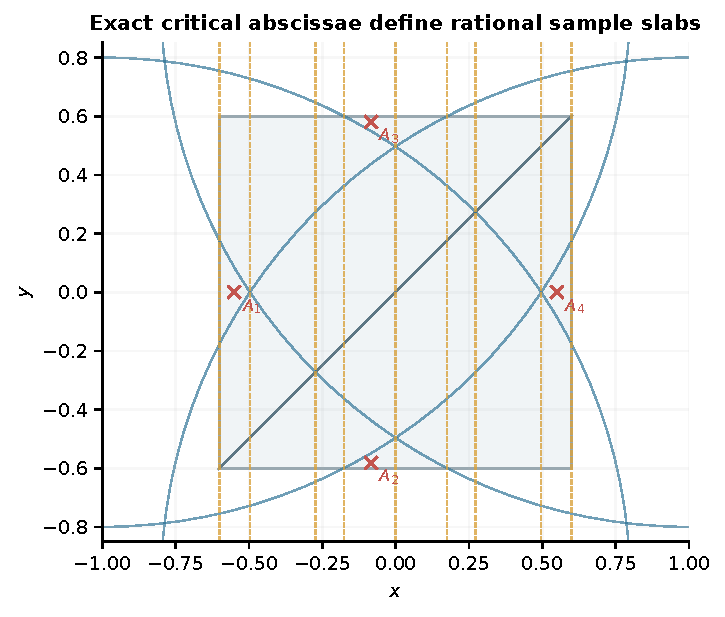
\includegraphics[width=\textwidth]{figures/vertical-slices.pdf}
\caption{Critical abscissae for the same panel. Open slabs contain no geometric ordering event. Rational samples between exact boundary ordinates recover the minimal contact labels without a raster resolution parameter.}
\end{figure}

\FloatBarrier
